%!TEX encoding=UTF-8 Unicode
%!TEX root=../thesis.tex

To evaluate \gls{Tabarnac}, we present two examples of benchmark optimization done with \gls{Tabarnac}.
For each benchmark, we compare the speedup obtained with \gls{Tabarnac} to the one obtained by \gls{NUMA} mapping tools.
We also evaluate the overhead of \gls{Tabarnac} on each of the \gls{NPB}.

\subsubsection{Methodology}

%This section briefly discusses our experimental setup for the evaluation of \gls{Tabarnac}.
% and presents relevant information on the experimental environment.
%presents the hardware architecture, the mapping policies to which we compare
%pour propositions, and the other relevant environment informations.

\begin{table}[htb]
    \centering
    \begin{tabular}{lccccc}
        \toprule
        & \multicolumn{5}{c}{\textbf{Totals}}\\
        \cmidrule(lr){2-6}
        & Nodes & Threads & Vendor & Model & Memory \\
        \cmidrule(lr){2-6}
        \texttt{Turing}   & $4$ & $64$ & Intel & Xeon X7550   & \SI{128}{Gib} \\
        \texttt{Idfreeze} & $8$ & $48$ & AMD   & Opteron 6174 & \SI{256}{Gib}\\
        \midrule
        & \multicolumn{5}{c}{\textbf{Per node}}\\
        \cmidrule(lr){2-6}
        & Cores & Threads & Frequency & L3 Cache & Memory \\
        \cmidrule(lr){2-6}
        \texttt{Turing}   & $8$ & $16$ & \SI{2.00}{Ghz}& \SI{18}{Mib} & \SI{32}{Gib} \\
        \texttt{Idfreeze} & $6$ & $6$  & \SI{2.20}{Ghz}& \SI{12}{Mib} & \SI{32}{Gib}\\
        \midrule
        & \multicolumn{5}{c}{\textbf{Software}}\\
        \cmidrule(lr){2-6}
        & Kernel & \multicolumn{2}{c}{Distribution} &
            \multicolumn{2}{c}{Bios configurations} \\
        \cmidrule(lr){2-6}
        \texttt{Turing}   & Linux 3.13 & \multicolumn{2}{c}{Ubuntu 12.04} &
            \multicolumn{2}{c}{Hyper threading} \\
        \texttt{Idfreeze} & Linux 3.2 & \multicolumn{2}{c}{Debian Jessie} &
            \multicolumn{2}{c}{No hyper threading}\\
        \bottomrule
    \end{tabular}
    \caption{Hardware and software configuration of the evaluation system for Tabarnac.}
    \label{tab:turing-hw}
\end{table}

We used two NUMA machines for our experiments, \texttt{Turing} and \texttt{Idfreeze}.
The second machine was only used to compare the instrumentation overhead on Intel and AMD machines, all the other experiments ran on \texttt{Turing}.
The hardware and software configurations are summarized in \tbl{turing-hw}.
%\texttt{Turing} runs version $3.13$ of the Linux kernel, while \texttt{Idfreeze} runs version $3.2$.

We evaluated the following applications with \gls{Tabarnac} in this paper: the \IS benchmark from the \gls{NPB} and \Ondes.
They were chosen to demonstrate different memory access behaviors with different strategies to improve them.

All applications use OpenMP for parallelization, they were compiled with \texttt{gcc}, version 4.6.3, with the \texttt{-O2} optimization flag.
Both analysis and performance evaluation are performed with $64$ threads, which is the maximum number of threads that our main evaluation machine (\texttt{Turing}) can execute in parallel.
%The \emph{matrix multiplication} performance was evaluated with
%matrices of size $4096 \times 4096$ doubles and $8192 \times 8192$, resulting on
%a memory usage of $128$Mib and $512Mib$ per matrix.
%\subsection{Mapping Policies}

In the performance evaluation, we compare the following three traditional mapping policies to the version modified using the knowledge provided by \gls{Tabarnac}.
The original \gls{Linux} kernel is our baseline for the experiments.
We use an unmodified Linux kernel, version $3.13$, with the first-touch policy.
The NUMA Balancing mechanism is disabled in this baseline.
The \emph{interleave} policy is performed with the help of the \texttt{numactl} tool~\cite{Kleen05NUMA}.
We also compare our results to the recently introduced \emph{NUMA Balancing} technique~\cite{Corbet12Toward}, which is executed with its default configuration.

For the plots presenting speedups, each configuration was executed at least $10$ times.
Each point shows the arithmetic mean of all runs.
The error bars in those plots represent the standard error.

All the files required to reproduce the experiments described here or the analysis are available online at: \url{https://github.com/dbeniamine/tabarnac\_expe}.

% \subsubsection{Matrix Multiplication}
%
% The first benchmark presented is based on a naive matrix multiplication,
% computing $C=A \times B$. Our aim here is not to provide a kernel competing with the
% state of the art, but to show how \gls{Tabarnac} can help to improve such
% applications. We compare two implementations of the matrix multiplication, in
% the first one, called \emph{Naive}, each thread starts by computing
% $C[0][tid]$ and then jumps $N$ elements after in the matrix, where $N$ is the
% number of threads. Although this implementation is known to be inefficient, it is a
% good example of NUMA-unaware code, and comparing the \gls{Tabarnac} visualization
% for this algorithm to the one obtained with a better version helps understanding
% how to interpret it.
% Moreover, when an application has such an unstructured memory access pattern, it
% is not always possible to change the pattern completely. Therefore, it is
% interesting to discuss the improvements that can be obtained in this kernel without
% modifying the algorithm.
% The optimized implementation of the matrix multiplication uses a non-recursive block
% decomposition.
%
%
%
% \begin{figure}[htb]
%     \centering
%     \begin{subfigure}{.49\linewidth}
%         \caption{Structure B (naive version).}
%         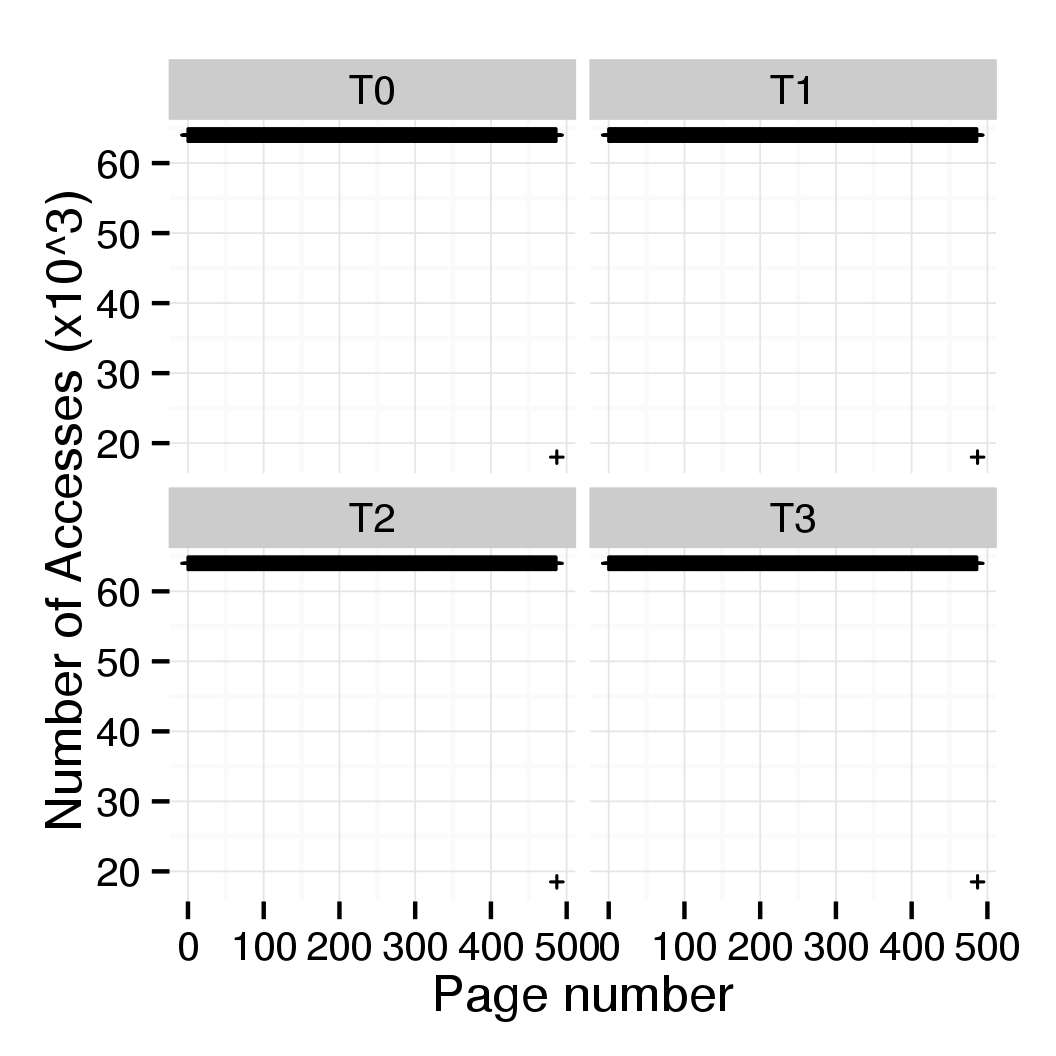
\includegraphics[width=\linewidth] {tabarnac/mat_B_modulo}
%         \label{fig:matrix-B-naive}
%     \end{subfigure}
%     \begin{subfigure}{.49\linewidth}
%         \caption{Structure C (naive version).}
%         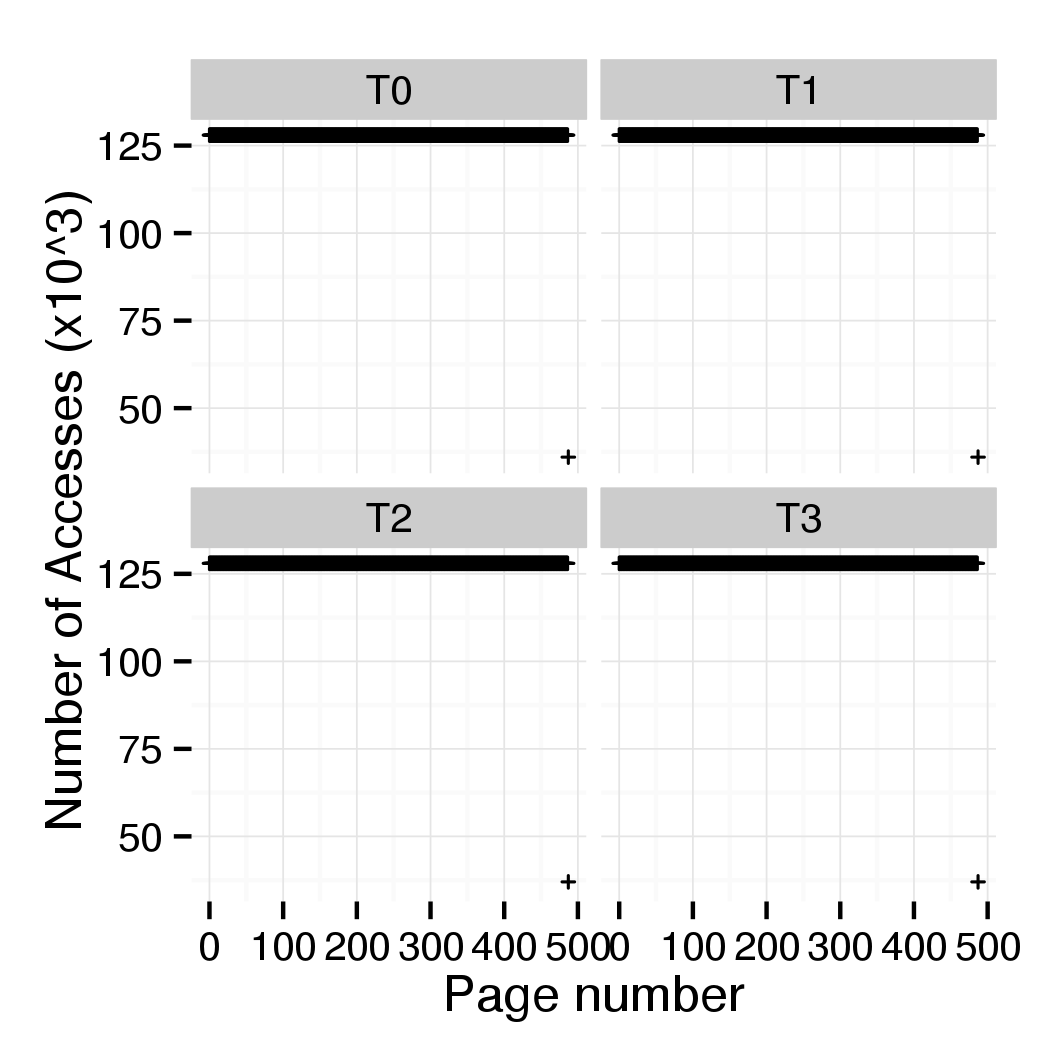
\includegraphics[width=\linewidth] {tabarnac/mat_C_modulo}
%         \label{fig:matrix-C-naive}
%     \end{subfigure}
%     \begin{subfigure}{.49\linewidth}
%         \caption{Structure B (block version).}
%         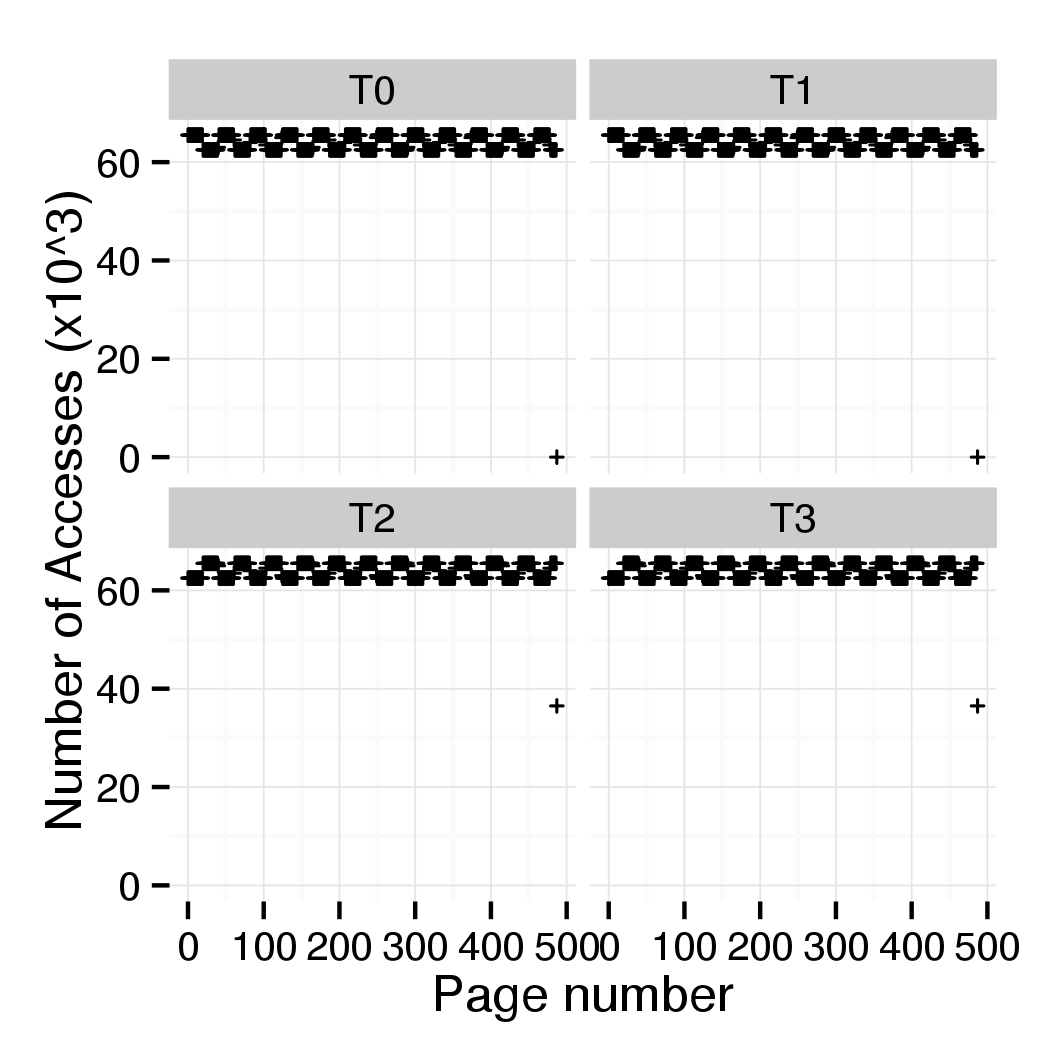
\includegraphics[width=\linewidth] {tabarnac/mat_B_bloc}
%         \label{fig:matrix-B-bloc}
%     \end{subfigure}
%     \begin{subfigure}{.49\linewidth}
%         \caption{Structure C (block version).}
%         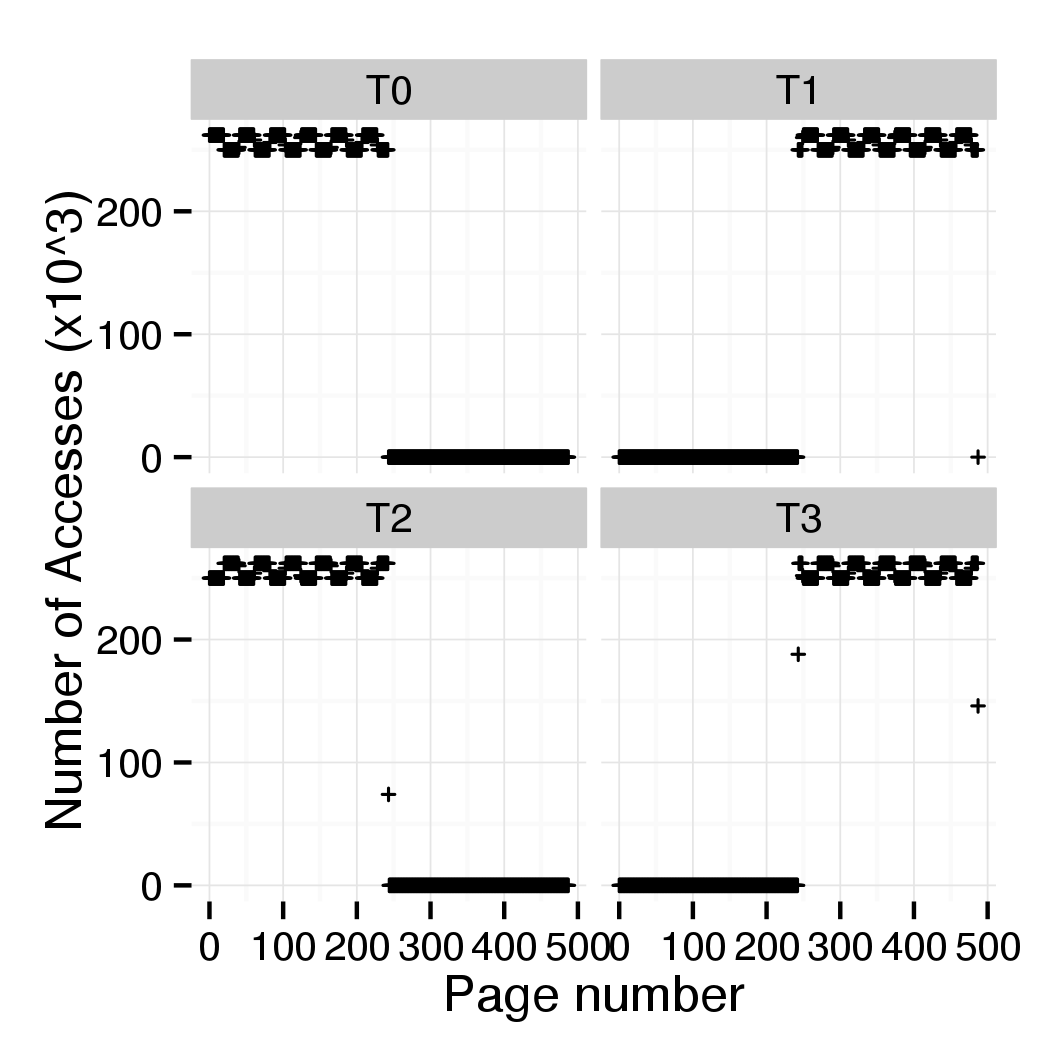
\includegraphics[width=\linewidth] {tabarnac/mat_C_bloc}
%         \label{fig:matrix-C-bloc}
%     \end{subfigure}
%     \caption{Per-thread access distribution on data structures B and C for the
%     matrix multiplication.}
%     \label{fig:matrix-analysis}
% \end{figure}
% % The figures presented in this sections are part of the \gls{Tabarnac} visualization.
% The analysis of the matrix multiplication is shown in \fig{matrix-analysis}.
% Each plot shows the number of memory accesses for a particular data structure
% per page and per thread. Only structures \texttt{B} and \texttt{C} are
% presented, since \texttt{A} has a very similar access
% pattern as \texttt{C} for both implementations.
% For the naive matrix multiplication, all pages of both structures are used by every
% thread, as we can see in
% Figures~\ref{fig:matrix-B-naive}~and~\ref{fig:matrix-C-naive}. Therefore, when we execute this code on a NUMA machine, wherever we
% map the page, all the nodes but one will trigger remote memory accesses. There
% are several ways to improve this behavior: an easy solution
% is to tell the operating system to interleave pages through the different
% nodes. This will result in a better balance of memory bandwidth between the
% nodes. Another solution is to create local copies of \texttt{A} and
% \texttt{B} on each node as these matrices are only read. Finally, we can modify
% the algorithm to improve the locality, which means using the block algorithm.
%
% \begin{figure}[htb]
%     \centering
%     \begin{subfigure}{.49\linewidth}
%         \caption{Structure B (block version).}
%         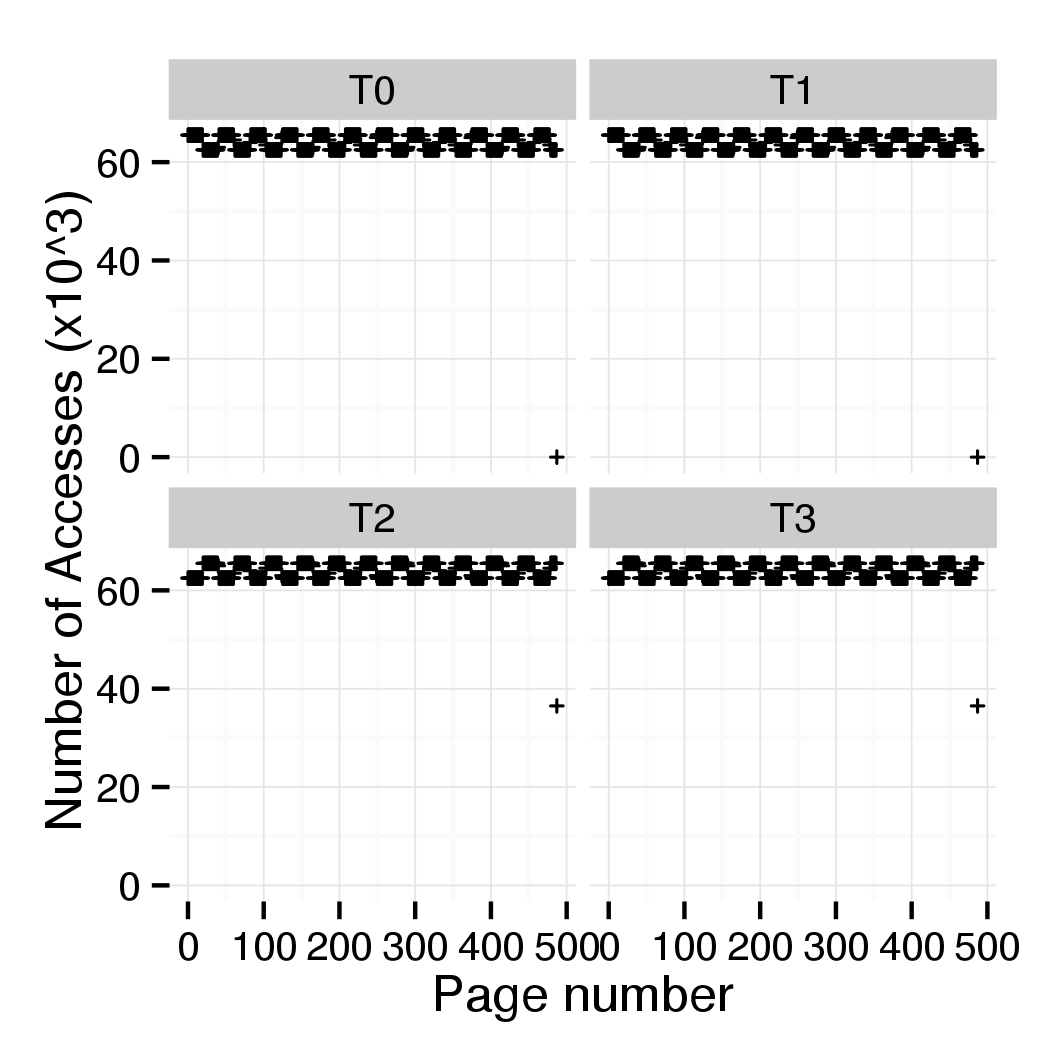
\includegraphics[width=\linewidth] {tabarnac/mat_B_bloc}
%         \label{fig:matrix-B-bloc}
%     \end{subfigure}
%     \begin{subfigure}{.49\linewidth}
%         \caption{Structure C (block version).}
%         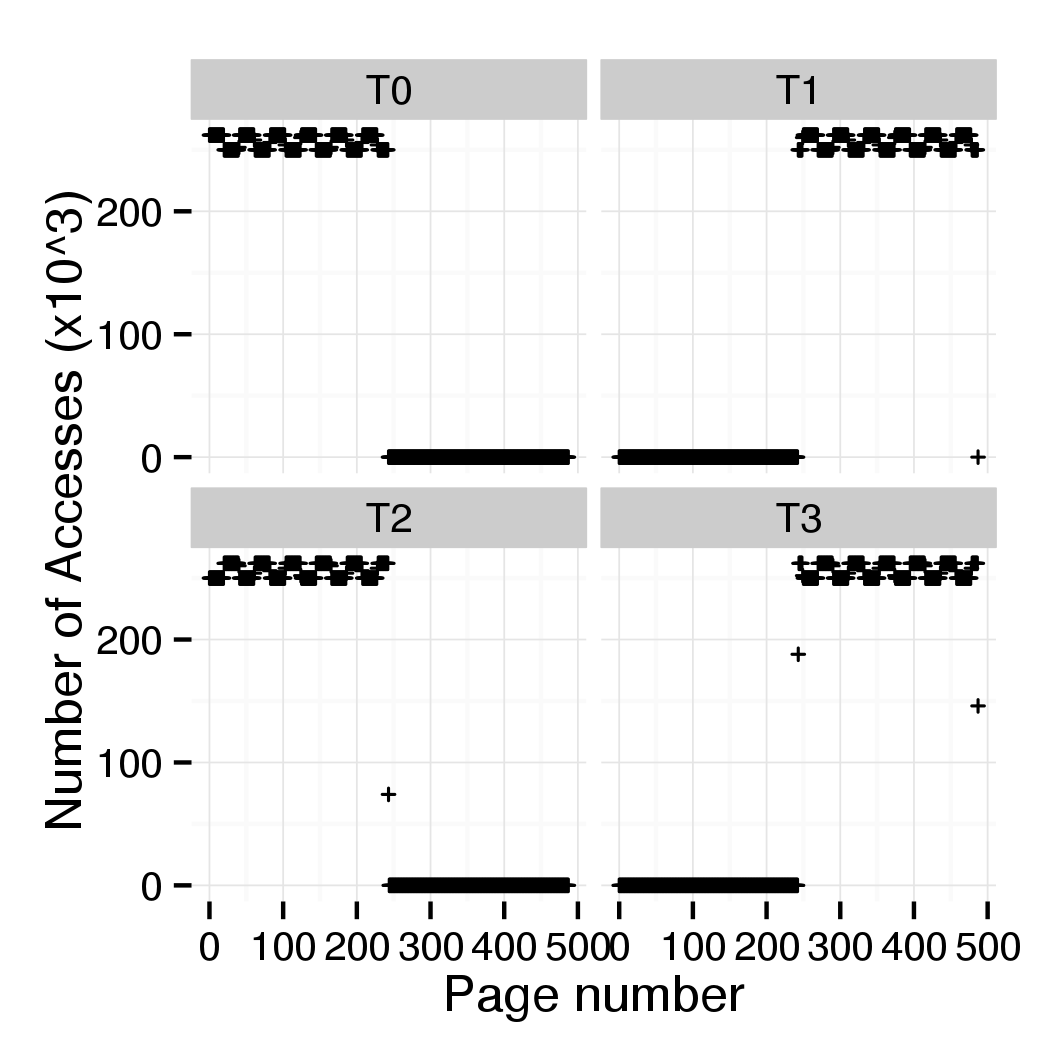
\includegraphics[width=\linewidth] {tabarnac/mat_C_bloc}
%         \label{fig:matrix-C-bloc}
%     \end{subfigure}
%     \caption{By thread access distribution on data structures A and B for the
%     block matrix multiplication.}
%     \label{fig:matrix-bloc}
% \end{figure}
%
% As we can see in Figures~\ref{fig:matrix-B-bloc}~and~\ref{fig:matrix-C-bloc}, the block algorithm improves the page
% locality compared to the naive implementation. In our algorithm, structures \texttt{B}
% and \texttt{C} are not divided the same way, resulting in two different access patterns. For structure \texttt{B} (\fig{matrix-B-bloc}), the pages still
% have similar numbers of accesses for all threads. Structures \texttt{C} and
% \texttt{A} (\fig{matrix-C-bloc}) are split in two parts. The first half
% is shared by threads $T0$ and $T2$ while the two others work on the second
% half. This behavior provides strong page locality and is therefore more
% suitable for NUMA machines. We can easily put each part of \texttt{C} (and
% \texttt{A}) on a NUMA node and map the threads using them to this node, while matrix
% \texttt{B} can be distributed using an interleave policy.
%
% To evaluate the performance improvements of the proposed modifications, we compare the execution
% time of both versions of the code (naive and block) with the mapping suggested by \gls{Tabarnac} to the original Linux kernel (base), and to NUMA Balancing.
% For the naive version, the interleave policy is identical to \gls{Tabarnac} and is therefore not shown separately.
% We use bigger matrix for the block version than for the naive one as this
% algorithm is designed to benefit from cache and thus reduce the impact of NUMA
% mapping policy.
%
%
% \begin{figure}[htb]
%     \centering
%     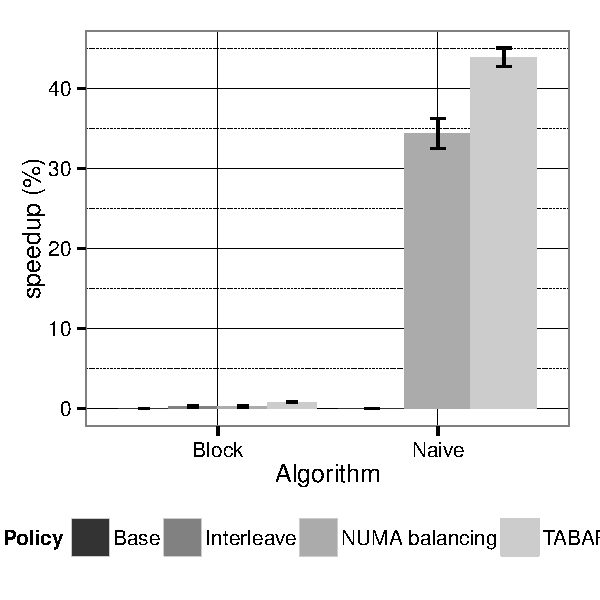
\includegraphics[width=\linewidth]{tabarnac/mat_time}
%     \caption{Speedup of the matrix multiplication for size $4096 \times 4096$
%     doubles (naive) and size $8192 \times 8192$ doubles (block).}
%     \label{fig:matrix-res}
% \end{figure}
%
% \fig{matrix-res} shows the experimental results of the matrix multiplication. We can see that for
% the naive algorithm, NUMA Balancing is already quite efficient and results in a \SI{40}{\%}
% speedup. However, using the \gls{Tabarnac} policy avoids the runtime overhead and
% allows us to obtain almost \SI{50}{\%} of speedup. For the block version, even with
% matrix $4$ times bigger, all policies provide similar execution times, as this
% algorithm is designed to fit in the caches of the system, such that the NUMA
% policy should not influence the results.
%
% This example shows
% how \gls{Tabarnac} can help improving an application by highlighting an inefficient
% memory access behavior. This knowledge can be used two different ways, and always
% results in significant performance improvements. Either the user can modify the code to
% improve the access distribution (in this case going from the naive to the block version),
% or at least \gls{Tabarnac} will help choosing the best NUMA page mapping policy.

\subsubsection{Ondes3D}
\label{sec:exp-ondes3d}

\Ondes is the main numerical kernel of the Ondes3D application~\cite{Dupros08Exploiting}.
It simulates the propagation of seismic waves using a finite-differences numerical method.
\Ondes has a memory usage of \SI{11.3}{Gib} with the parameters used for the performance evaluation, and \SI{0.7}{Gi}b for the analysis.

\begin{figure}[htb]
    \centering
    \begin{subfigure}{.49\linewidth}
        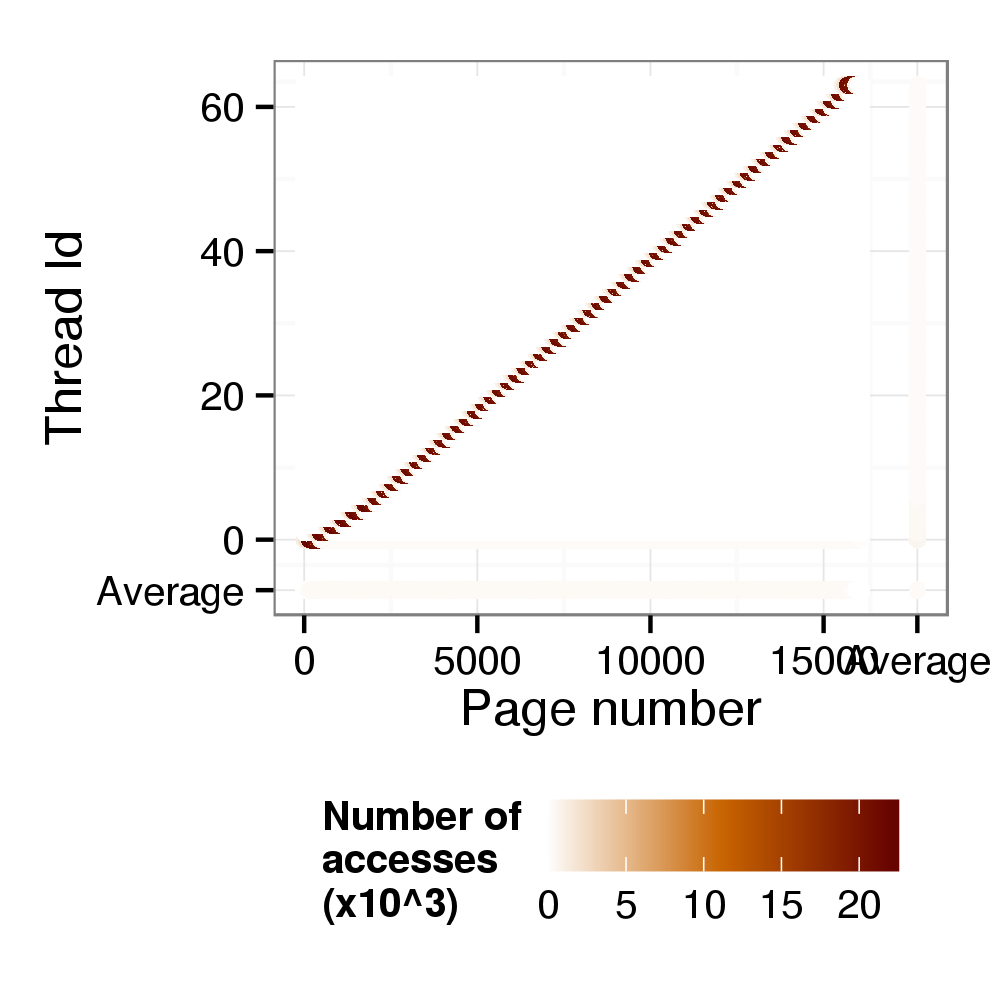
\includegraphics[width=\linewidth] {tabarnac/ondes3d_vz0_dist_orig}
        \caption{Access distribution}
        \label{fig:ondes3d-behaviour-vz0-orig}
    \end{subfigure}
    \newline
    \begin{subfigure}{.49\linewidth}
        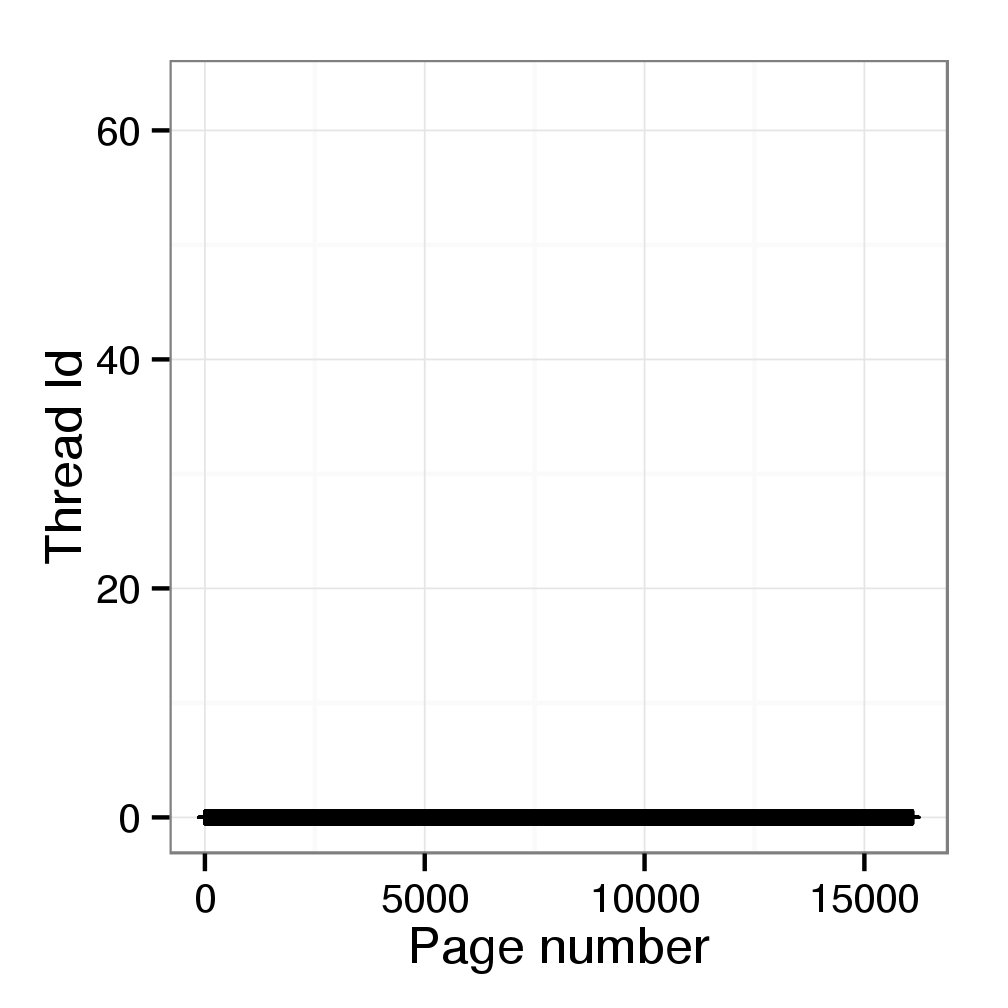
\includegraphics[width=\linewidth] {tabarnac/ondes3d_vz0_ft_orig}
        \caption{Original first-touch.}
        \label{fig:ondes3d-ft-vz0-orig}
    \end{subfigure}
    \begin{subfigure}{.49\linewidth}
        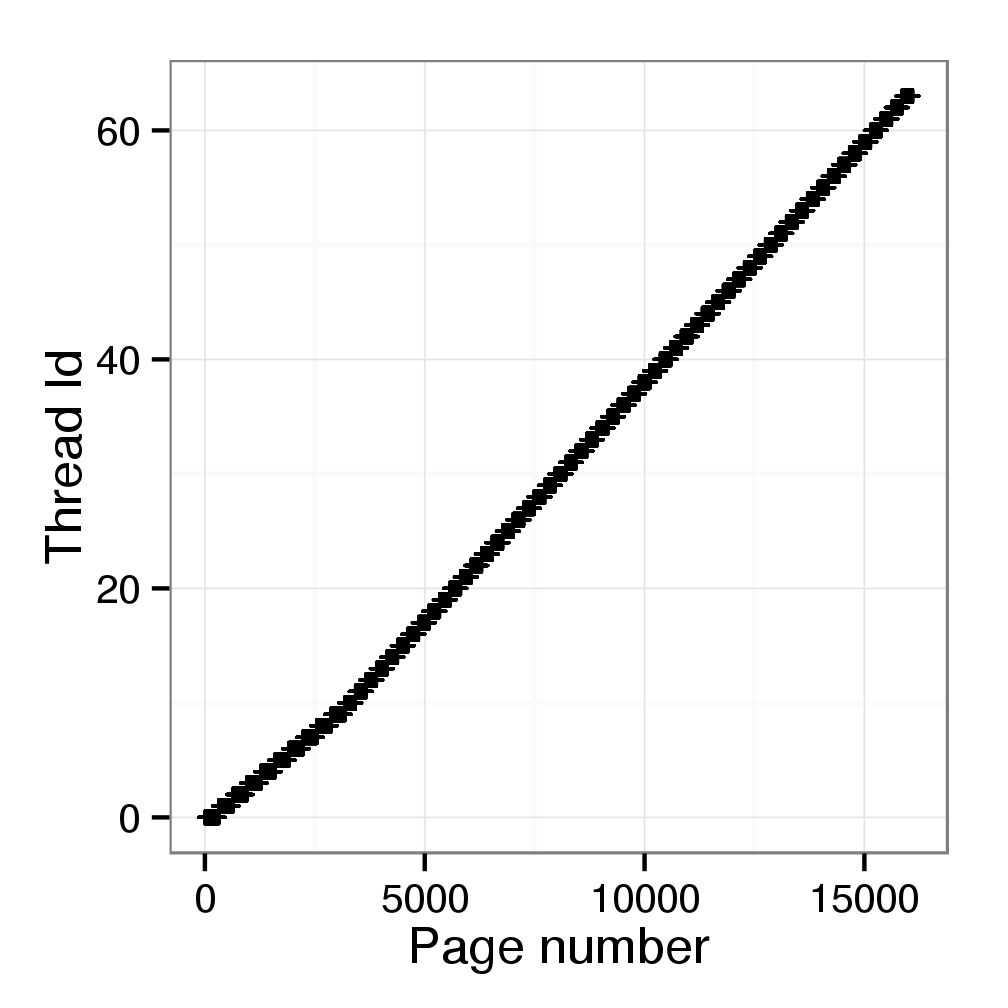
\includegraphics[width=\linewidth] {tabarnac/ondes3d_vz0_ft_modif}
        \caption{Improved first-touch.}
        \label{fig:ondes3d-ft-vz0-modif}
    \end{subfigure}
    \caption{Access distribution and first-touch for structure
        \texttt{vz0} from \Ondes.} %Original version on the left,
    %modified on the right.}
    \label{fig:ondes3d}
\end{figure}

The analysis of the accesses distribution in \Ondes shows that each structure seems to be well distributed between the threads, as we can see for structure \texttt{vz0} in \fig{ondes3d-behaviour-vz0-orig}.
However, for all structures, thread~$0$ is responsible for all first accesses, as we can see in \fig{ondes3d-ft-vz0-orig}.
Due to this pattern, if we run \Ondes without any improved mapping policy, every page will be mapped to the \gls{NUMA} node that executes the thread~$0$, resulting in mostly remote
accesses for the other threads.
An easy fix is to perform the initialization in parallel and to pin each thread on a different core.
Such a modification results in the first touch distribution shown in \fig{ondes3d-ft-vz0-modif}, for which pages are distributed among all the threads.

\begin{figure}[htb]
    \centering
    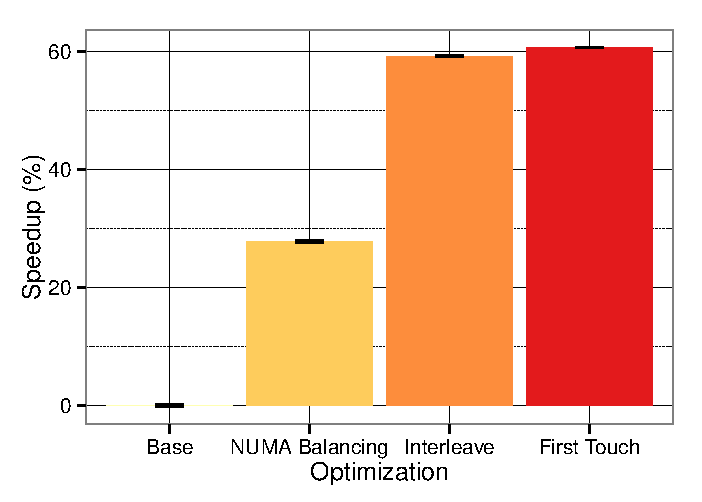
\includegraphics[width=.7\linewidth]{tabarnac/ondes3d_exectime}
    \caption[Speedup for \Ondes.]{Speedup for \Ondes compared to the baseline.}
    \label{fig:ondes-res}
\end{figure}

We compare the performance of the modified version called \emph{First Touch} to the original (\emph{Base}) version, both running on the normal OS.
We also evaluate the use of \emph{NUMA Balancing} that move pages online and \emph{Interleave} policy that aims at reducing the impact of remote accesses.
\fig{ondes-res} present the results of this evaluation.
We can see that all methods improve the execution time compared to the \gls{OS}.
Still, but \emph{NUMA Balancing} provides less than \SI{30}{\%} speedup, while the static mappings (Interleave and the modified code) increase performance by \SI{60}{\%}.
Indeed, with \emph{NUMA Balancing}, all pages are initially mapped by the \gls{OS} to the \gls{NUMA} node of thread~$0$, and are only moved later on, after many remote accesses have already occurred, losing some optimization opportunities.
This is a case where static mapping can be substantially better than automated tools.
The \emph{Interleave} policy provides a similar speedup as \emph{First Touch} since it distributes the pages over the \gls{NUMA} nodes at the beginning of the execution.
In the end, for this example, using a classic static policy would have been enough to fix the performance issue, yet \gls{Tabarnac} helped understanding and fixing it in a definitive way.

\subsubsection{The \IS benchmark}


% We executed \gls{Tabarnac} on the benchmarks %written in \texttt{C}
% from the OpenMP
% implementation of the \gls{NPB}~\cite{Jin99NPBOpenMP}.
% %\tod{there are just 2...}
% % David: Actually we tried also some fortran NPB but I didn't insist on
% % getting the good structure names as the access patterns were ``good''
% Most
% of them have either a well balanced accesses pattern between the threads or a
% totally random accesses distribution. For all of them, the first touch fits exactly
% the access distribution. However, the analysis of \IS caught our attention.
% \IS sorts a set of integer numbers using a parallel bucket sort
% algorithm.
According to the \gls{NPB} website\footnote{\url{http://www.nas.nasa.gov/publications/npb.html}}, \IS has a random memory access pattern, while we observed a very specific pattern.
In this section we explain this pattern and how we used it to improve the performance of \IS.

\IS was executed with input class \emph{D} for the performance evaluation, resulting in a memory usage of \SI{33.5}{Gib}, and class \emph{B}\footnote{
    \DC was run in class \emph{A} as it was too slow in class \emph{B} to run the full experiment.}
    for the analysis, with a memory usage of \SI{0.25}{Gib}.

\begin{figure}[htb]
    \centering
    \begin{subfigure}{.4\linewidth}
        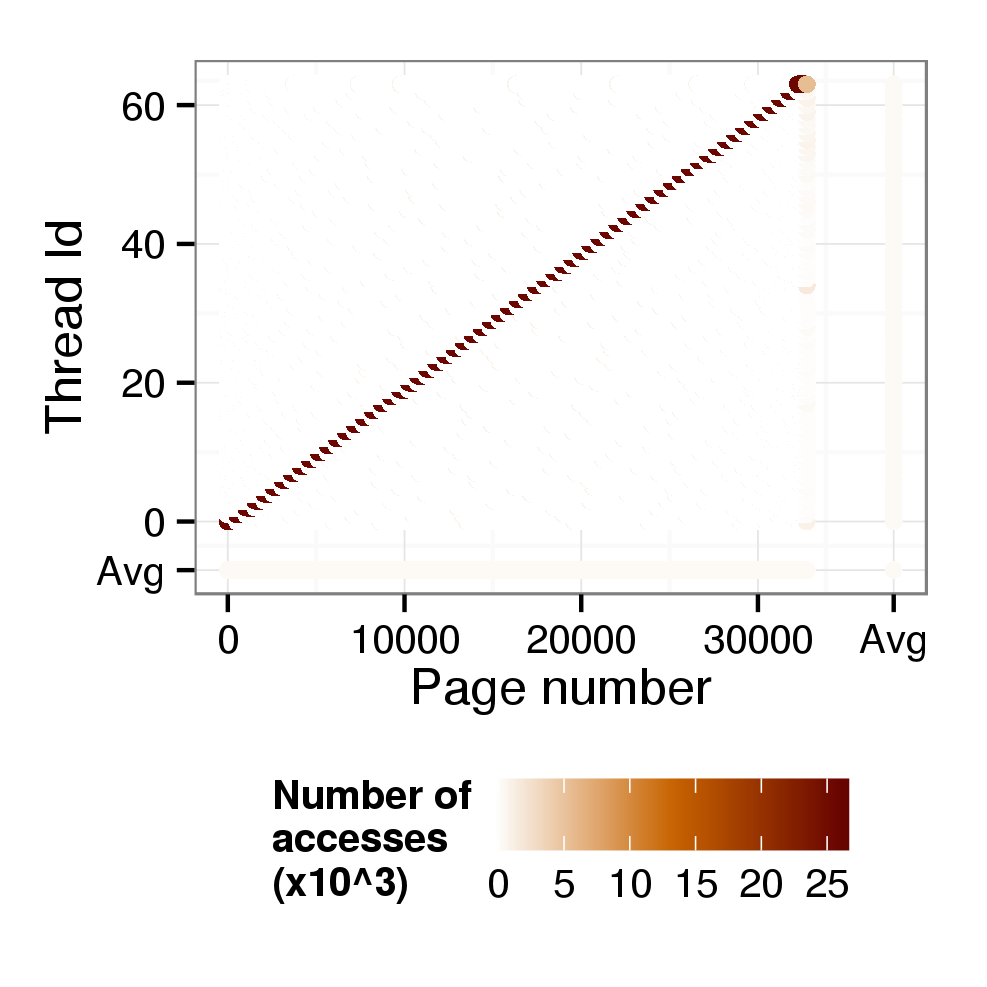
\includegraphics[width=\linewidth]  {tabarnac/is_b_kba_orig}
        \caption{\texttt{key\_array}.}
        \label{fig:is-behaviour-orig-kba}
    \end{subfigure}
    ~
    \begin{subfigure}{.4\linewidth}
        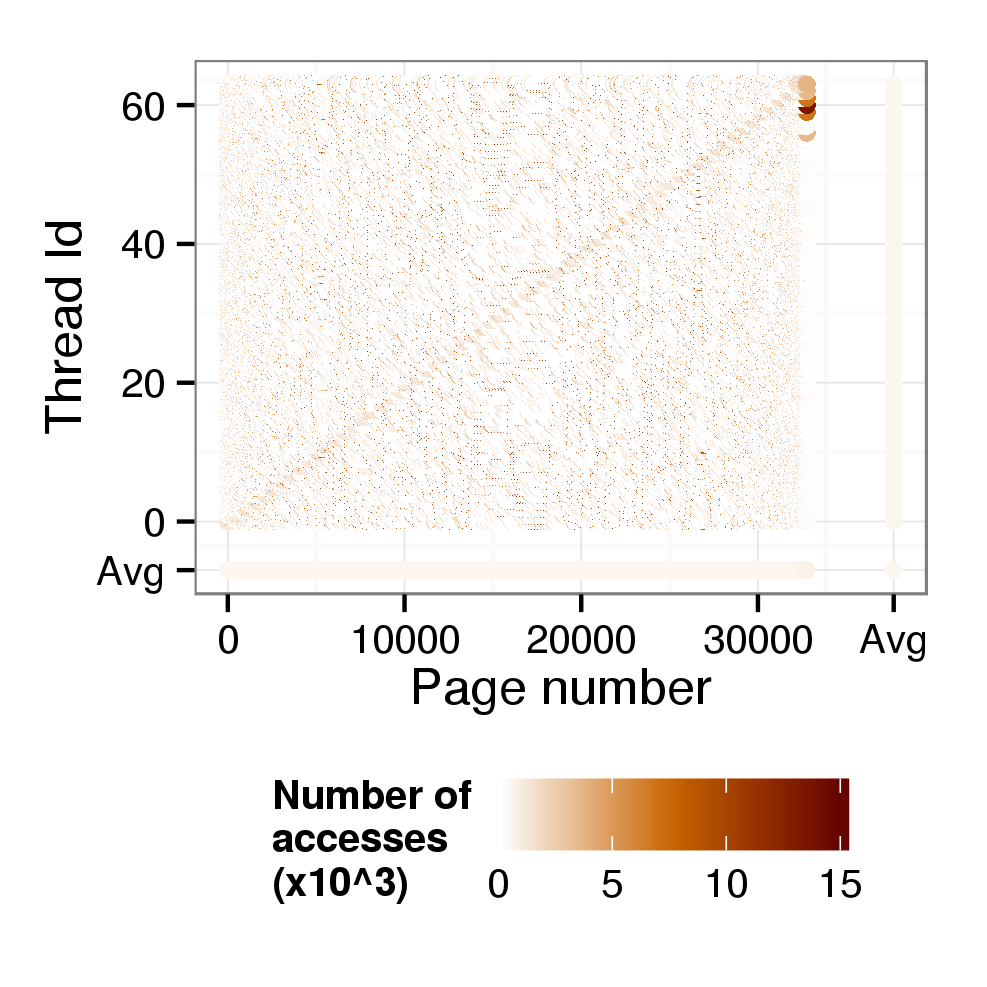
\includegraphics[width=\linewidth]  {tabarnac/is_b_kb2_orig}
        \caption{\texttt{key\_buff2}.}
        \label{fig:is-behaviour-orig-kb2}
    \end{subfigure}
    \begin{subfigure}{.4\linewidth}
        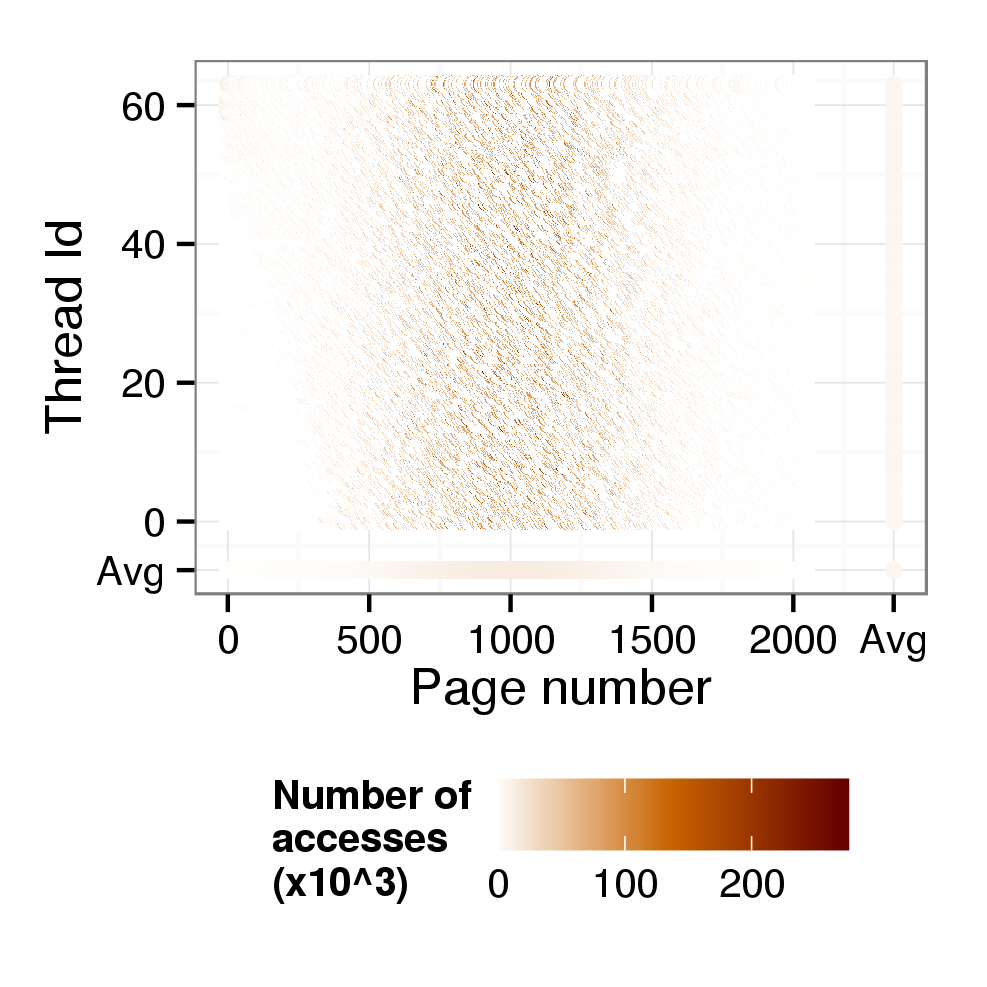
\includegraphics[width=\linewidth]  {tabarnac/is_b_kb1_orig}
        \caption{\texttt{key\_buff1}.}
        \label{fig:is-behaviour-orig-kb1}
    \end{subfigure}
    \caption[Original memory access distribution for \IS.]{Original memory access distribution for the main structures of \IS.}
    \label{fig:is-behaviour-orig}
\end{figure}

\fig{is-behaviour-orig} shows the original access distributions for the three main structures of \IS.
We can see that each structure has a different access pattern: for \texttt{key\_array} (\fig{is-behaviour-orig-kba}) each thread works on a different part of the structure, which permits automated tools perform an efficient data/thread mapping on it.
On the other hand, \texttt{key\_buff2} (\fig{is-behaviour-orig-kb2}) is completely shared by all threads, we can barely see a diagonal pattern, indicating a small affinity between some threads and some pages.
\texttt{key\_buff1}'s access distribution (\fig{is-behaviour-orig-kb1}) is the most interesting one.
We can see that almost all accesses occur in pages in the middle of the structure (from page $500$ to $1500$), and those pages are shared by all threads.
This means that the number of access per page  for each thread follows a Gaussian distribution centered in the middle of the structure.

\lstinputlisting[caption={[Original IS code.]\IS code responsible for the distribution of memory accesses.}, label=lst:is, float=htb]{code/is.c}

We can identify the source of this pattern in the \IS source code.
Indeed, all the accesses to \texttt{key\_buff1} are linear, except the ones shown in \lstr{is}\footnote{
    The code has been slightly modified to make it more readable.
    In the original version, the arrays generic pointers.
    Furthermore we removed several lines of code inside the loop that are not required to understand the memory pattern.
    }, Line~\ref{lst:is-gaus-end}, which depend on the values of \texttt{key\_buff2}.
Those accesses happens in an \gls{OpenMP} parallel loop that has the particularity to be scheduled dynamically.
The comments on the \IS code explains that the values of \texttt{key\_buff2} follows a Gaussian distribution, therefore using a dynamic scheduling provides a good load balancing between the threads, while a cyclic distribution would results in some threads generating significantly more memory accesses than the others.
Still it is possible to use a cyclic scheduling instead of the default one (dynamic) by defining a variable at the compilation time.

\begin{lstlisting}[caption={Modified IS code.}, label=lst:is-modif,float=htb]
#pragma omp for schedule(static,NUM_BUCKETS/
    (2*omp_get_num_threads()))
\end{lstlisting}

As simple cyclic distribution of the loop would result in unbalanced work, we can design a slightly more complex distribution keeps a good load balancing while enforcing locality of data.
To do so, we split the loop into two equal parts and distribute each part among the threads in a cyclic way.
This can be done by modifying the \gls{OpenMP} pragma (Line~\ref{lst:is-sched} in the original code), as shown in \lstr{is-modif}.

\begin{figure}[htb]
    \centering
    \begin{subfigure}{.4\linewidth}
        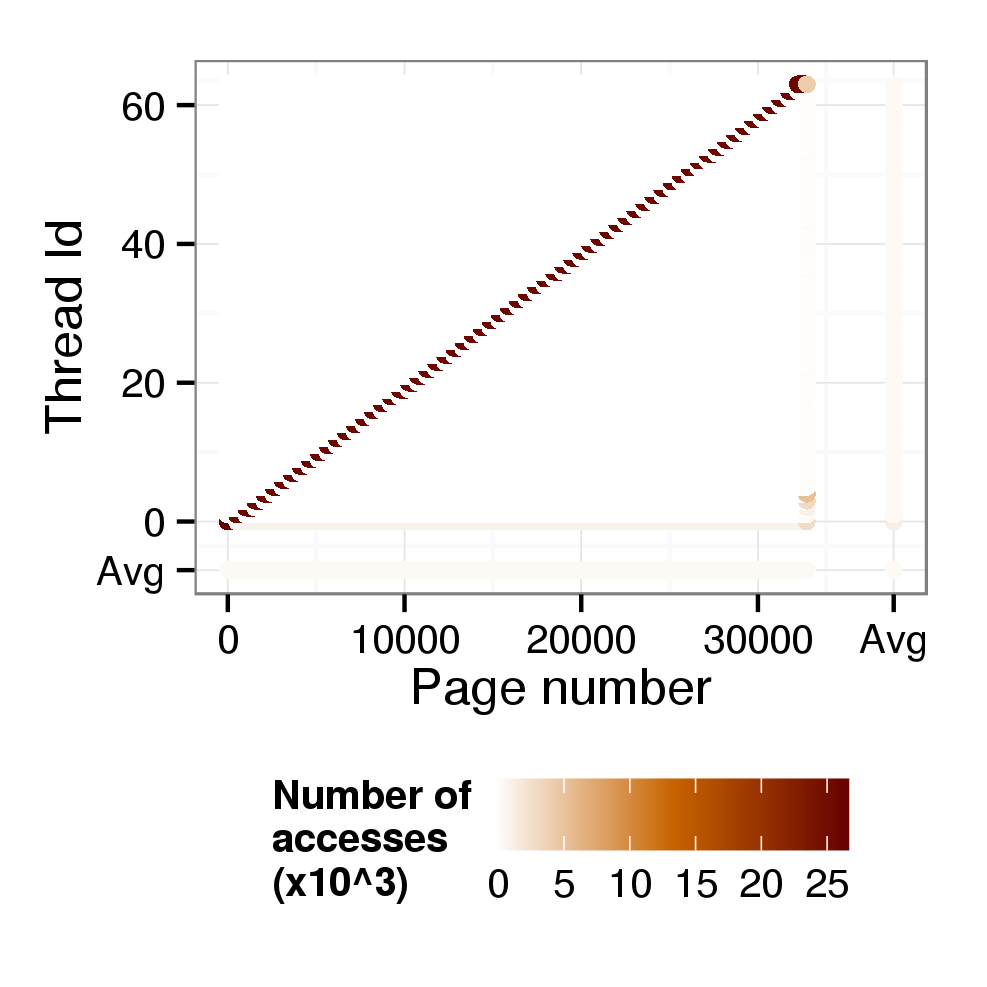
\includegraphics[width=\linewidth] {tabarnac/is_b_kba_modif}
        \caption{\texttt{key\_array}.}
        \label{fig:is-behaviour-modif-kba}
    \end{subfigure}
    ~
    \begin{subfigure}{.4\linewidth}
        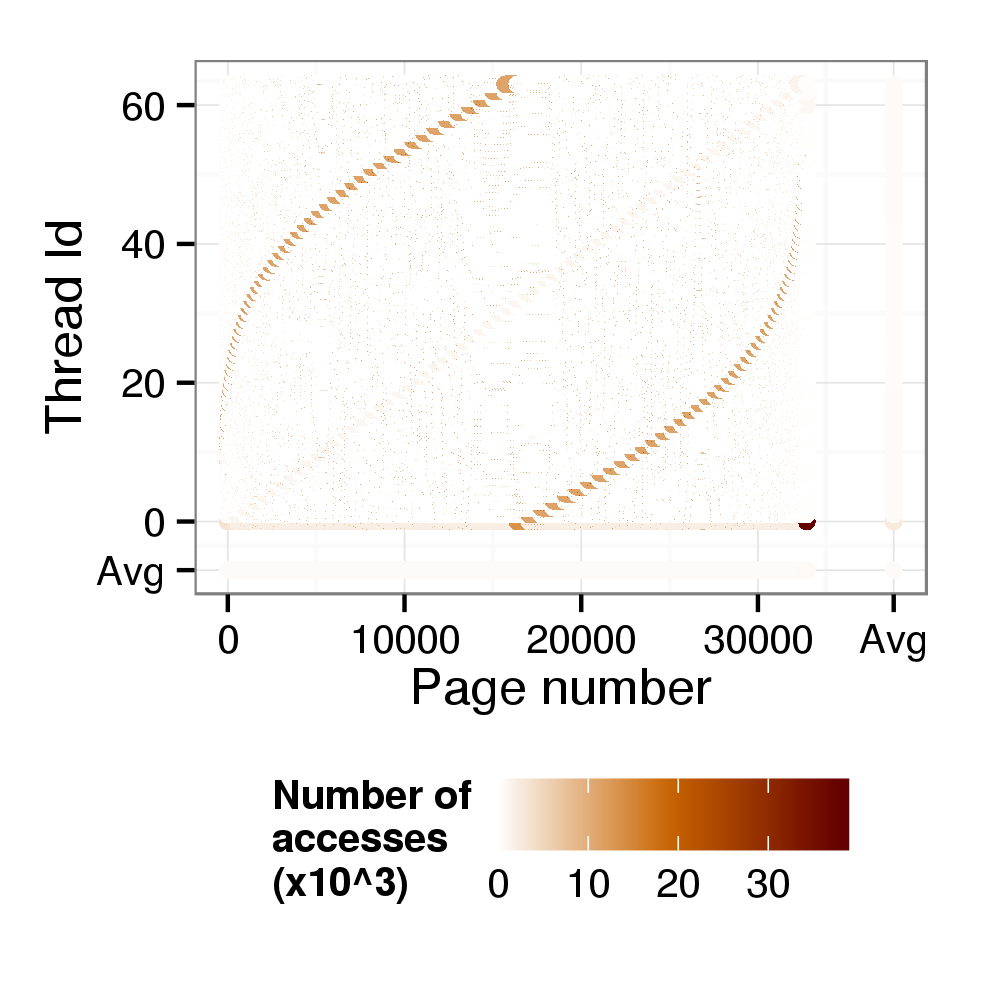
\includegraphics[width=\linewidth] {tabarnac/is_b_kb2_modif}
        \caption{\texttt{key\_buff2}.}
        \label{fig:is-behaviour-modif-kb2}
    \end{subfigure}
    \begin{subfigure}{.4\linewidth}
        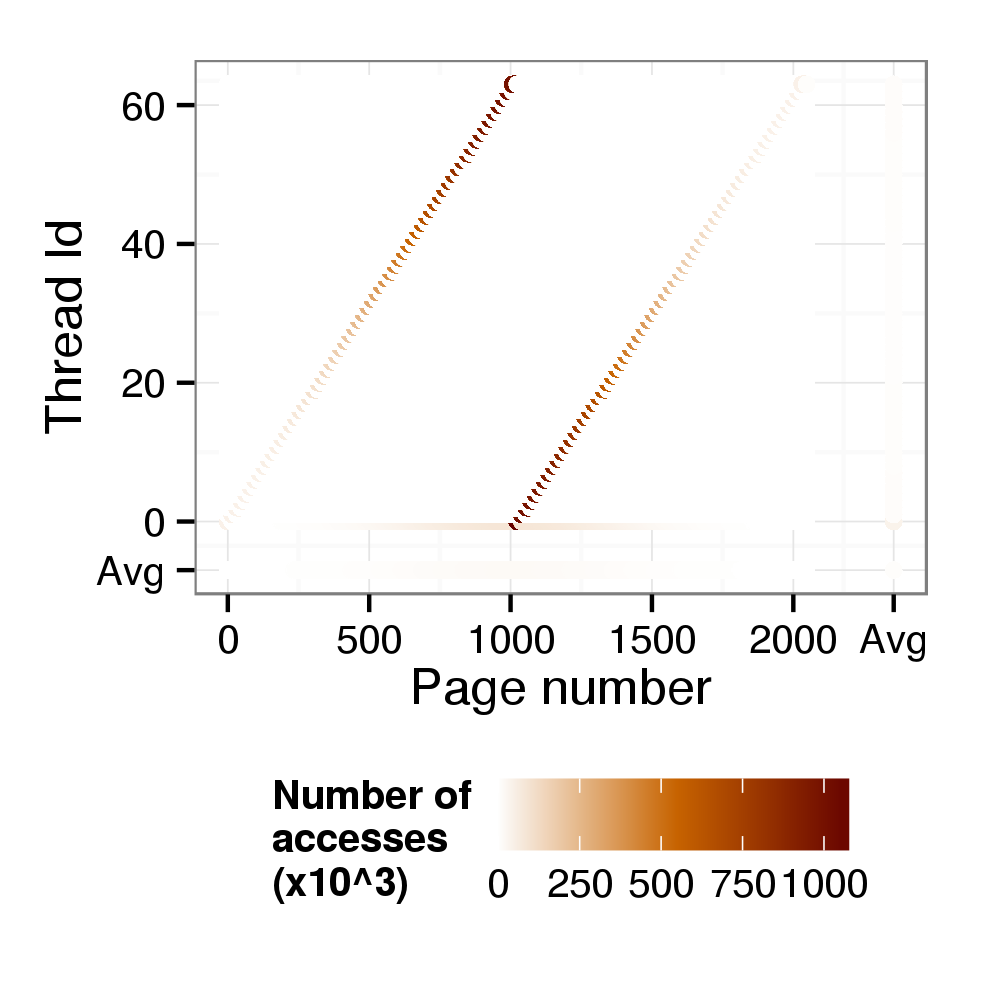
\includegraphics[width=\linewidth] {tabarnac/is_b_kb1_modif}
        \caption{\texttt{key\_buff1}.}
        \label{fig:is-behaviour-modif-kb1}
    \end{subfigure}
    \caption[Modified memory access distribution for \IS.]{Modified memory access distribution for the main structures of \IS.}
    \label{fig:is-behaviour-modif}

\end{figure}



With this code modification, we obtain the access distribution shown in \fig{is-behaviour-modif}.
We can see that now each thread accesses a different part of \texttt{key\_buff1}.
Furthermore, if most of the accesses still occur in the middle of the structure, the average number of access across the structure is the same for all threads, which means that our distribution preserves the good load balancing.
Our modification has also changed \texttt{key\_buff2}'s accesses distribution.
Indeed, we can now clearly see a sharing pattern very similar to the one obtained for \texttt{key\_buff1}.

The main point of our code modification is to improve the affinity between thread and memory, therefore we need to pin each thread on a core to keep them close to the data they access.
To perform the thread mapping, we use the \texttt{GOMP\_CPU\_AFFINITY} environment variable.
\gls{Tabarnac} also showed us that the first touch is always done by the thread actually using the data for IS, therefore we do not need to explicitly map the data to the \gls{NUMA} nodes.

We compare the execution time of \IS (class \emph{D}) for the three scheduling methods, \emph{Dynamic}, \emph{Cyclic} and \emph{Cyclic-Split}: cyclic with the proposed distribution.
For the two first methods, we compare the execution time on the base operating system, the interleave policy and with \gls{NUMA} balancing enabled.
As we map threads manually, interleave and \gls{NUMA} Balancing are not relevant with our modifications and are therefore not evaluated.

\begin{figure}[htb]
    \centering
    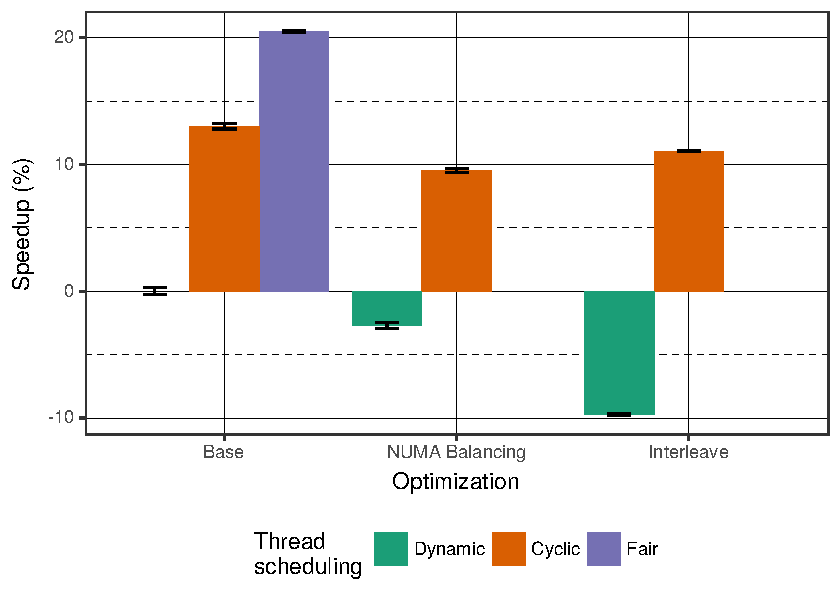
\includegraphics[width=\linewidth]{tabarnac/is_exectime}
    \caption[Speedup for \IS.]{Speedup for \IS (class D) compared to the baseline.}
\label{fig:is-res}
\end{figure}

\fig{is-res} shows the speedup of \IS compared to the default version (\emph{Dynamic}) for each scheduling method and for each optimization technique.
The first thing to notice is that with the default \emph{Dynamic} scheduling, both Interleave and \gls{NUMA} Balancing slow the application down, by up to \SI{10}{\%}.
This slowdown is due to the fact that two mechanisms (the mapping policy and the \gls{OpenMP} runtime) or modifying the application behavior with conflicting interests and without communicating.
Then we can note that \emph{Cyclic} scheduling, proposed in the original code, already provides up to \SI{13}{\%} of speedup.
Yet, both interleave and \gls{NUMA} Balancing are still reducing the performance gains.
Finally, the \emph{Cyclic-Split} version provides more than \SI{20}{\%} of speedup with a very small code modification.
This example shows that while mapping policies (static or dynamic) can conflict with the parallel runtime and slow the execution time, analyzing an application's memory behavior can help fixing inefficient behavior resulting in significant performances gain.

\subsubsection{Tracing overhead}

Finally,  we evaluate the instrumentation cost of \gls{Tabarnac}.
To do so, we executed all of the \gls{NPB} in class \emph{B} with $64$ threads on both evaluation systems and compared the original execution time to the execution time with instrumentation enabled.

\begin{figure}[htb]
    \centering
    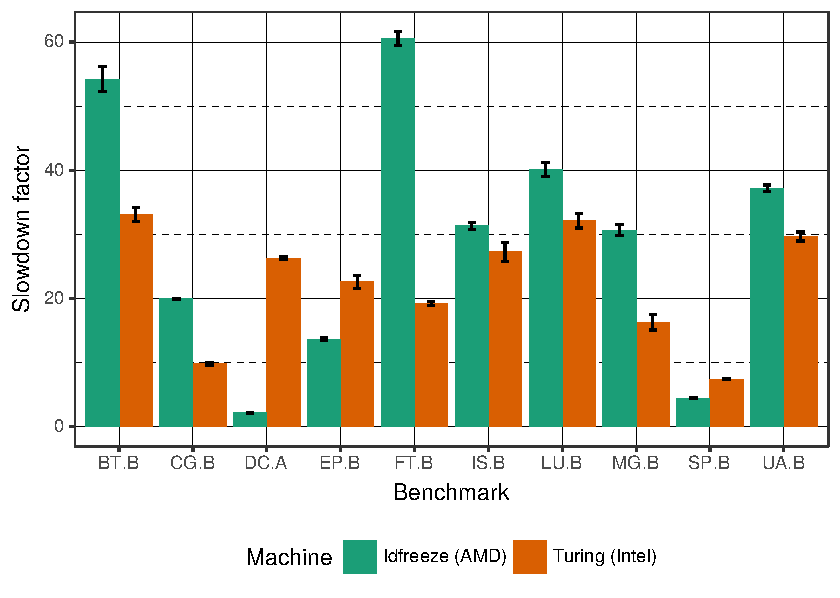
\includegraphics[width=\linewidth]{tabarnac/tool-ovh.pdf}
    \caption{Tabarnac's instrumentation overhead.}
    \label{fig:ovh-tabarnac}
\end{figure}

As we can see in \fig{ovh-tabarnac}, on the Intel machine, the instrumentation slows the execution down by a factor from $10$ to $30$.
On the \gls{AMD} machine, the instrumentation is $10$ to \SI{50}{\%} slower for most benchmarks, and two to three times slower than on the \gls{Intel} machine for pathological cases.
Although this overhead is not negligible, we have to consider the fact that often we can instrument smaller versions of the applications, as we focus on the general behavior.
Finally, as our analysis is designed to be used during the development phase and at runtime in an automated tool, we consider that this overhead is acceptable.


\subsection{Results and discussion}

Our experiments have highlighted the fact that both static mapping policies such as Interleave and dynamic tools such as \gls{NUMA} Balancing can either provide performance gain or loss.
Furthermore sometimes one tool is significantly more efficient than the other.
The only way to predict which tool is the most suited to an application is to understand the sharing patterns of the memory of this application by the threads.

\gls{Tabarnac} enables developers and users to achieve performance improvements in two ways.
First, by providing a deep understanding of the memory sharing pattern, it enables the user to find the best mapping policy.
Second, this knowledge can be used to identify and fix inefficient memory behavior.
Our experiments showed that both situations result in significant performance gains.

While \gls{Tabarnac} helps to identify and fix some inefficient sharing patterns, it only provides a global overview of the memory usage.
Indeed it does not collect any temporal information.
Therefore, it does not enable identification of inefficient memory access patterns over the time, such as the ones depicted in \sect{archi} with the naïve matrix multiplication.

% vim: et si sta lbr  sw=4 ts=4 spelllang=en_us
